\section{Introduction}\label{sec:intro}

\begin{figure}[!t]
  \centering  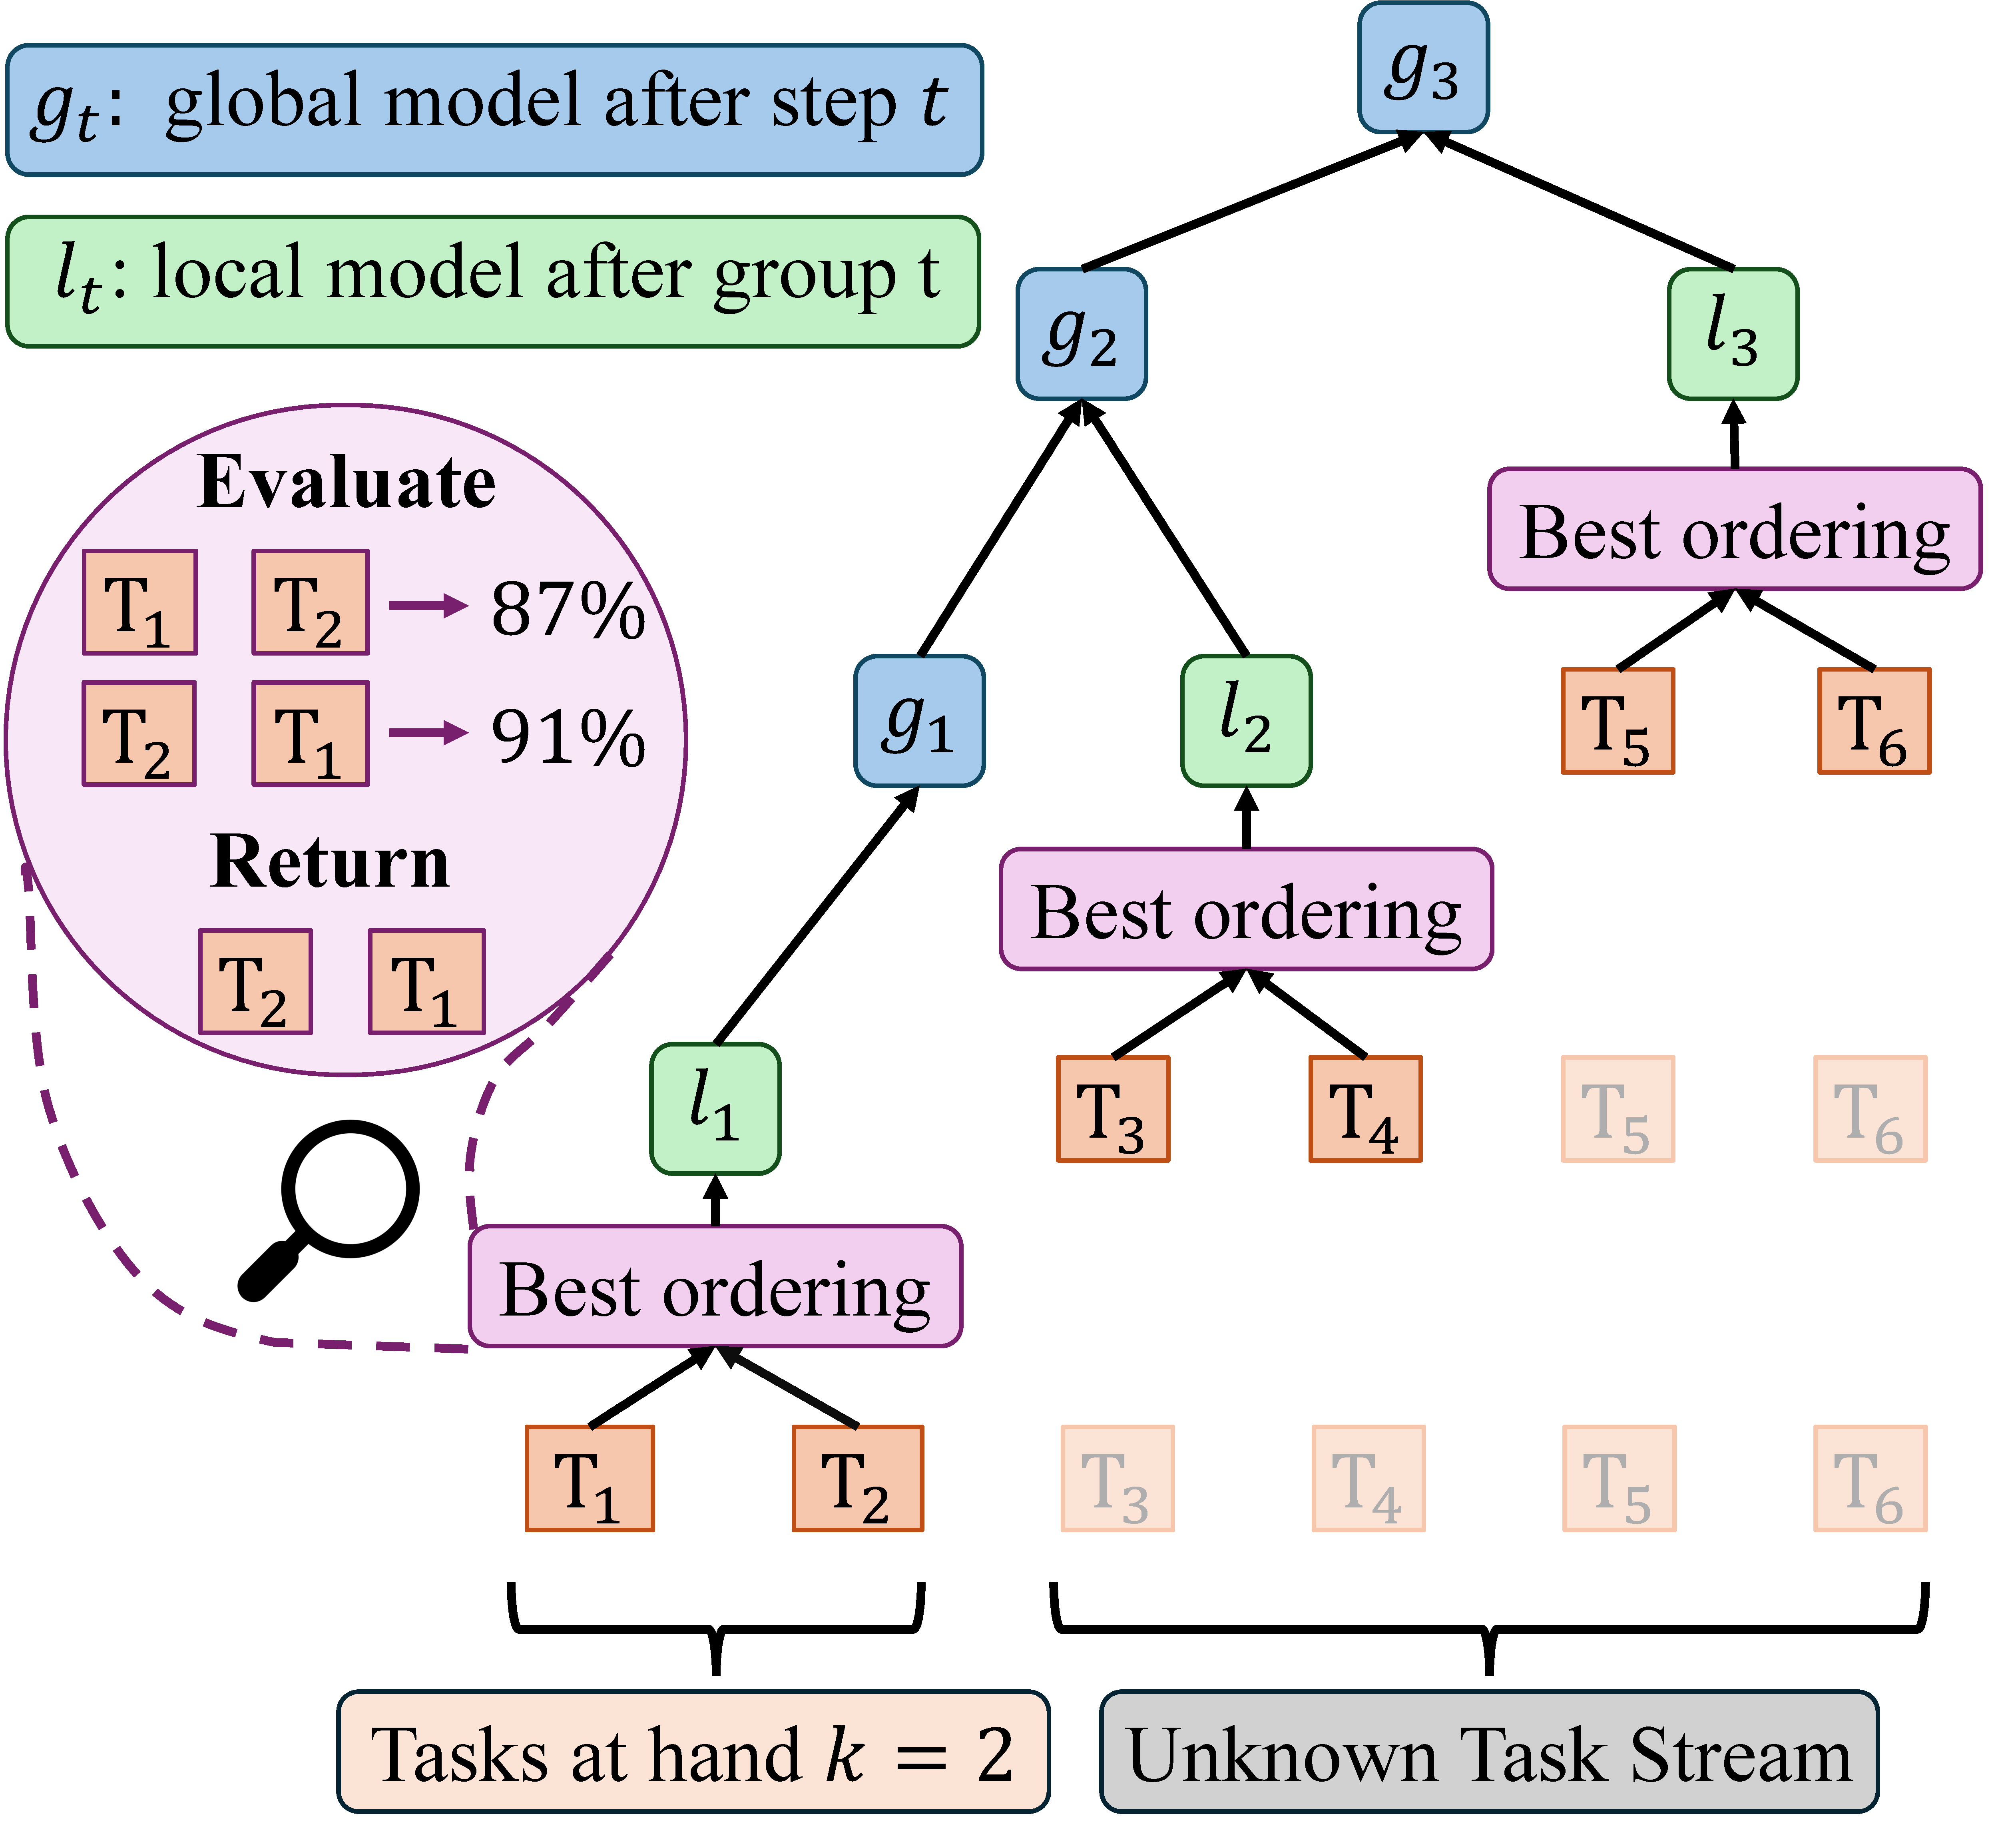
\includegraphics[width=\columnwidth]{figures/hier-explanation-fig.pdf}
  \caption{\textbf{Overview of HTCL with group size $k=2$.} The task stream is partitioned into disjoint groups (faded tasks denote the future stream)}
  \label{fig:hier-explanation}
\end{figure}

Continual learning (CL) aims to enable neural networks to acquire knowledge sequentially without catastrophically forgetting previously learned information~\cite{kirkpatrick2017overcoming, parisi2019continual}. This capability,  studied extensively~\cite{rebuffi2017icarl, zenke2017continual, fernando2017pathnet}, encounters a fundamental challenge: \emph{task-order sensitivity}. In particular, empirical studies report substantial increases in performance variance, up to $22\%$, in real-world deployments, where task sequences are rarely under the practitioner’s control~\cite{de2021continual} (see Appendix~\ref{app:impact-example} and related experiments in~\cite{bell2022effect, riemer2018learning}). %

\emph{Such variance is unacceptable in practice}. For instance, a medical diagnosis model's performance cannot depend on the order in which the diseases are introduced to it during training. A naive solution to this problem is to train the model over all possible task orderings and select the best one. However, such exhaustive training is NP-hard since $n$ tasks will require training the model on $n!$ permutations. \emph{Therefore, it is infeasible to find the best order of tasks over which to train.}

\begin{figure}[!t]
  \centering
  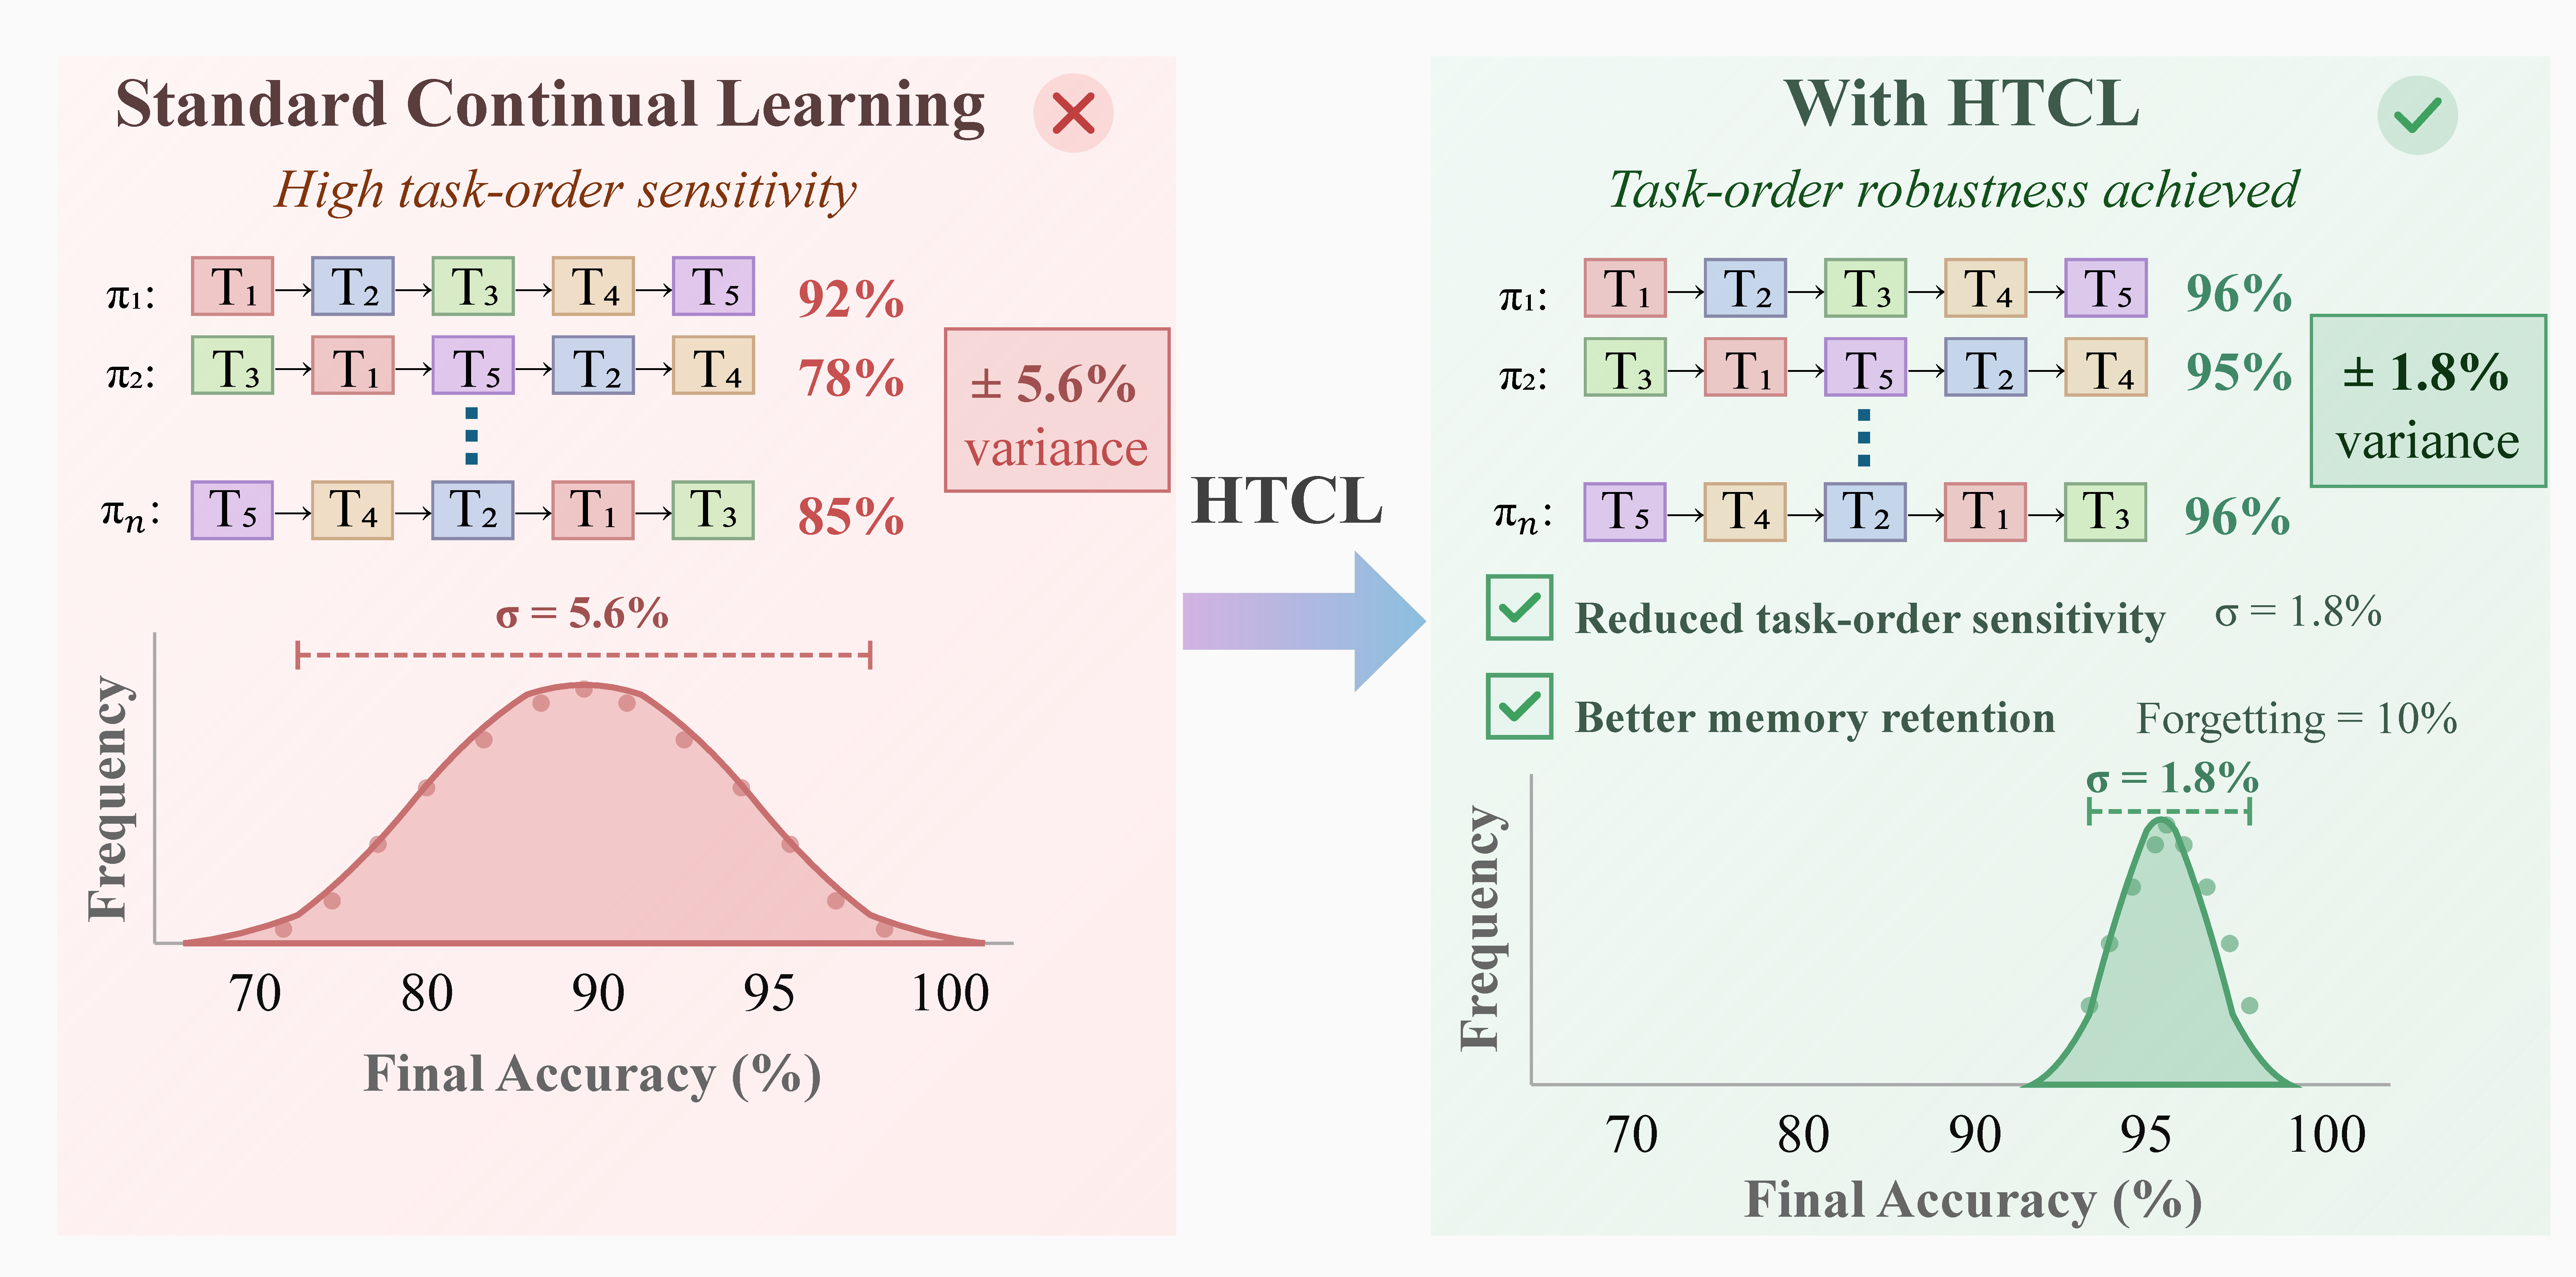
\includegraphics[width=\columnwidth]{figures/first-page.pdf}
  \caption{Task-order sensitivity in CL and its mitigation via HTCL. \textbf{Left:} Standard CL methods exhibit high sensitivity to task ordering. \textbf{Right:} HTCL achieves consistent performance regardless of task ordering, producing a narrow accuracy distribution.}
  \label{fig:new-cl-goal}
\end{figure}
Alternatively, it is more attractive to understand ``\emph{how to increase the robustness of the model in the presence of arbitrary task order?}"  To this end, we introduce \textbf{Hierarchical Taylor Series-based Continual Learning (HTCL)}. Our hierarchical framework imagines two levels of sequential consolidation steps as shown in Figure \ref{fig:hier-explanation}. At the first level, we collect $k$ tasks from the CL task sequence. Using these $k$ tasks, we determine the best task order and train a local model. Next, at level 2, we collect two local models from level one and consolidate them using a second order update rule. This consolidated model is then used as the initial condition for the next sequence of $k$ tasks, and the two-level training process is repeated. This simple two-step approach incorporates two integral strategies, \emph{a divide and conquer strategy and a hierarchical consolidation strategy.} %

As illustrated in Figure \ref{fig:hier-explanation}, in the first level, our approach focuses on a small group of $k$ tasks collected online. Within these $k$ tasks, HTCL is \emph{model- and CL-method-agnostic}: one may employ any existing CL method, utilize any model architectures, and work on any sequence length. %
The information from multiple groups of $k$ is consolidated hierarchically through a Hessian-regularized Taylor expansion using low-rank curvature approximations that considers the sensitivity of the loss function to task order while performing updates.

\textbf{Empirically}, these features enable two consistent benefits across CL methods, data modalities, model type and scale. First, HTCL reduces task-order sensitivity: two-level HTCL reduces standard deviation of final accuracy by $33\text{--}68\%$ on SplitMNIST and $17\text{--}21\%$ on CIFAR-100, with SER + HTCL achieving a $67.86\%$  reduction (see Fig.~\ref{fig:ser-results}), these benefits extend to other modalities, yielding standard deviation reductions of approximately $33\textbf{--}38\%$ on graph (CORA) and text (20 Newsgroups) classification tasks. Second, HTCL improves memory retention: mean forgetting drops by up to $70.9\%$ (DER + HTCL on SplitMNIST); per-task standard deviation reduces by over $30\%$ in longer task sequences (see Fig.~\ref{fig:extended} for CIFAR-100 dataset). Ablations studies confirm the second-order term is essential: first-order and DiLoCo-style alternatives both degrade accuracy and amplify task-order variance (Appendix~\ref{app:fo-diloco}). We complement these empirical observations with formal theoretical guarantees from Theorem~\ref{thm:perf-bound-main} and Proposition~\ref{thm:tradeoff-main}. 

\textbf{Contribution:} Our contributions are fourfold. First, we identify \emph{task-order sensitivity} as a critical and under-addressed challenge in CL, where performance variance reaches up to $22\%$ in real-world deployments. Second, we propose a two-level divide-and-conquer approach that locally optimizes task order over small groups of $k$ tasks and consolidates hierarchically. Third, we establish theoretical guarantees for the framework. Fourth, we empirically validate HTCL across diverse modalities and scales indicating substantial improvement confirming that the second-order term is essential.

 

